% Created by tikzDevice version 0.12.3.1 on 2021-12-17 00:24:29
% !TEX encoding = UTF-8 Unicode
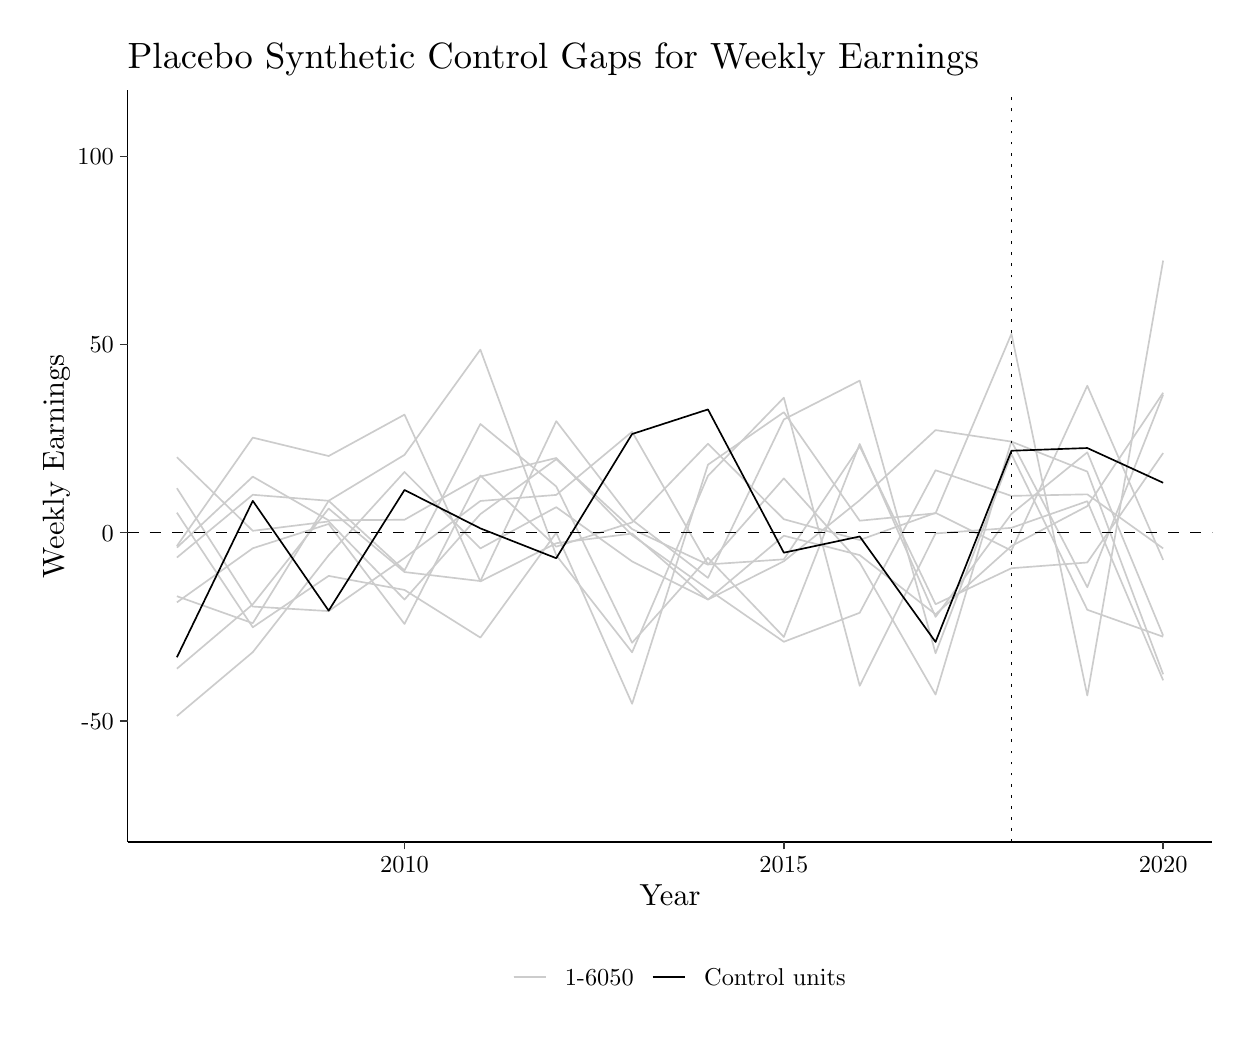
\begin{tikzpicture}[x=1pt,y=1pt]
\definecolor{fillColor}{RGB}{255,255,255}
\path[use as bounding box,fill=fillColor,fill opacity=0.00] (0,0) rectangle (433.62,361.35);
\begin{scope}
\path[clip] (  0.00,  0.00) rectangle (433.62,361.35);
\definecolor{drawColor}{RGB}{255,255,255}
\definecolor{fillColor}{RGB}{255,255,255}

\path[draw=drawColor,line width= 0.6pt,line join=round,line cap=round,fill=fillColor] (  0.00,  0.00) rectangle (433.62,361.35);
\end{scope}
\begin{scope}
\path[clip] ( 36.11, 67.14) rectangle (428.12,338.69);
\definecolor{drawColor}{gray}{0.80}

\path[draw=drawColor,line width= 0.6pt,line join=round] ( 53.93,129.72) --
	( 81.34,152.98) --
	(108.76,187.57) --
	(136.17,164.64) --
	(163.58,161.38) --
	(191.00,219.16) --
	(218.41,183.49) --
	(245.82,162.53) --
	(273.24,219.79) --
	(300.65,233.80) --
	(328.06,135.29) --
	(355.48,207.25) --
	(382.89,151.00) --
	(410.30,141.26);

\path[draw=drawColor,line width= 0.6pt,line join=round] ( 53.93,173.47) --
	( 81.34,199.11) --
	(108.76,183.32) --
	(136.17,183.54) --
	(163.58,199.13) --
	(191.00,205.85) --
	(218.41,177.94) --
	(245.82,158.43) --
	(273.24,139.44) --
	(300.65,149.92) --
	(328.06,201.43) --
	(355.48,192.16) --
	(382.89,192.72) --
	(410.30,173.17);

\path[draw=drawColor,line width= 0.6pt,line join=round] ( 53.93,174.06) --
	( 81.34,213.21) --
	(108.76,206.56) --
	(136.17,221.52) --
	(163.58,161.26) --
	(191.00,175.06) --
	(218.41,178.55) --
	(245.82,154.72) --
	(273.24,177.77) --
	(300.65,170.76) --
	(328.06,149.37) --
	(355.48,174.04) --
	(382.89,188.45) --
	(410.30,229.42);

\path[draw=drawColor,line width= 0.6pt,line join=round] ( 53.93,153.68) --
	( 81.34,173.23) --
	(108.76,182.01) --
	(136.17,145.88) --
	(163.58,199.52) --
	(191.00,173.81) --
	(218.41,182.58) --
	(245.82,210.98) --
	(273.24,183.73) --
	(300.65,176.22) --
	(328.06,186.03) --
	(355.48,172.40) --
	(382.89,231.96) --
	(410.30,169.04);

\path[draw=drawColor,line width= 0.6pt,line join=round] ( 53.93,155.90) --
	( 81.34,146.15) --
	(108.76,190.40) --
	(136.17,206.98) --
	(163.58,245.00) --
	(191.00,170.68) --
	(218.41,135.64) --
	(245.82,199.41) --
	(273.24,227.65) --
	(300.65,123.55) --
	(328.06,178.59) --
	(355.48,180.61) --
	(382.89,190.23) --
	(410.30,125.52);

\path[draw=drawColor,line width= 0.6pt,line join=round] ( 53.93,186.08) --
	( 81.34,144.68) --
	(108.76,163.25) --
	(136.17,158.17) --
	(163.58,140.95) --
	(191.00,178.82) --
	(218.41,117.03) --
	(245.82,203.43) --
	(273.24,222.40) --
	(300.65,183.19) --
	(328.06,185.86) --
	(355.48,250.71) --
	(382.89,120.02) --
	(410.30,277.19);

\path[draw=drawColor,line width= 0.6pt,line join=round] ( 53.93,206.15) --
	( 81.34,179.54) --
	(108.76,182.92) --
	(136.17,154.70) --
	(163.58,185.58) --
	(191.00,205.41) --
	(218.41,180.16) --
	(245.82,167.32) --
	(273.24,198.48) --
	(300.65,168.04) --
	(328.06,120.37) --
	(355.48,211.92) --
	(382.89,159.15) --
	(410.30,228.75);

\path[draw=drawColor,line width= 0.6pt,line join=round] ( 53.93,169.88) --
	( 81.34,192.56) --
	(108.76,190.39) --
	(136.17,165.20) --
	(163.58,218.14) --
	(191.00,195.56) --
	(218.41,139.09) --
	(245.82,169.76) --
	(273.24,141.18) --
	(300.65,210.91) --
	(328.06,148.44) --
	(355.48,185.65) --
	(382.89,207.90) --
	(410.30,141.66);

\path[draw=drawColor,line width= 0.6pt,line join=round] ( 53.93,194.93) --
	( 81.34,152.16) --
	(108.76,150.53) --
	(136.17,169.74) --
	(163.58,190.32) --
	(191.00,192.51) --
	(218.41,215.34) --
	(245.82,167.38) --
	(273.24,169.23) --
	(300.65,210.07) --
	(328.06,153.00) --
	(355.48,166.02) --
	(382.89,168.09) --
	(410.30,207.63);

\path[draw=drawColor,line width= 0.6pt,line join=round] ( 53.93,112.61) --
	( 81.34,135.69) --
	(108.76,170.70) --
	(136.17,200.81) --
	(163.58,173.17) --
	(191.00,188.08) --
	(218.41,168.48) --
	(245.82,154.71) --
	(273.24,168.54) --
	(300.65,190.58) --
	(328.06,215.93) --
	(355.48,211.77) --
	(382.89,200.94) --
	(410.30,127.70);
\definecolor{drawColor}{RGB}{0,0,0}

\path[draw=drawColor,line width= 0.6pt,dash pattern=on 1pt off 3pt ,line join=round] (355.48, 67.14) -- (355.48,338.69);

\path[draw=drawColor,line width= 0.6pt,dash pattern=on 4pt off 4pt ,line join=round] ( 36.11,178.87) -- (428.12,178.87);

\path[draw=drawColor,line width= 0.6pt,line join=round] ( 53.93,133.85) --
	( 81.34,190.37) --
	(108.76,150.69) --
	(136.17,194.29) --
	(163.58,180.42) --
	(191.00,169.64) --
	(218.41,214.51) --
	(245.82,223.40) --
	(273.24,171.63) --
	(300.65,177.49) --
	(328.06,139.38) --
	(355.48,208.47) --
	(382.89,209.45) --
	(410.30,196.90);
\end{scope}
\begin{scope}
\path[clip] (  0.00,  0.00) rectangle (433.62,361.35);
\definecolor{drawColor}{RGB}{0,0,0}

\path[draw=drawColor,line width= 0.6pt,line join=round] ( 36.11, 67.14) --
	( 36.11,338.69);
\end{scope}
\begin{scope}
\path[clip] (  0.00,  0.00) rectangle (433.62,361.35);
\definecolor{drawColor}{RGB}{0,0,0}

\node[text=drawColor,anchor=base east,inner sep=0pt, outer sep=0pt, scale=  0.88] at ( 31.16,107.87) {-50};

\node[text=drawColor,anchor=base east,inner sep=0pt, outer sep=0pt, scale=  0.88] at ( 31.16,175.84) {0};

\node[text=drawColor,anchor=base east,inner sep=0pt, outer sep=0pt, scale=  0.88] at ( 31.16,243.81) {50};

\node[text=drawColor,anchor=base east,inner sep=0pt, outer sep=0pt, scale=  0.88] at ( 31.16,311.78) {100};
\end{scope}
\begin{scope}
\path[clip] (  0.00,  0.00) rectangle (433.62,361.35);
\definecolor{drawColor}{gray}{0.20}

\path[draw=drawColor,line width= 0.6pt,line join=round] ( 33.36,110.90) --
	( 36.11,110.90);

\path[draw=drawColor,line width= 0.6pt,line join=round] ( 33.36,178.87) --
	( 36.11,178.87);

\path[draw=drawColor,line width= 0.6pt,line join=round] ( 33.36,246.84) --
	( 36.11,246.84);

\path[draw=drawColor,line width= 0.6pt,line join=round] ( 33.36,314.81) --
	( 36.11,314.81);
\end{scope}
\begin{scope}
\path[clip] (  0.00,  0.00) rectangle (433.62,361.35);
\definecolor{drawColor}{RGB}{0,0,0}

\path[draw=drawColor,line width= 0.6pt,line join=round] ( 36.11, 67.14) --
	(428.12, 67.14);
\end{scope}
\begin{scope}
\path[clip] (  0.00,  0.00) rectangle (433.62,361.35);
\definecolor{drawColor}{gray}{0.20}

\path[draw=drawColor,line width= 0.6pt,line join=round] (136.17, 64.39) --
	(136.17, 67.14);

\path[draw=drawColor,line width= 0.6pt,line join=round] (273.24, 64.39) --
	(273.24, 67.14);

\path[draw=drawColor,line width= 0.6pt,line join=round] (410.30, 64.39) --
	(410.30, 67.14);
\end{scope}
\begin{scope}
\path[clip] (  0.00,  0.00) rectangle (433.62,361.35);
\definecolor{drawColor}{RGB}{0,0,0}

\node[text=drawColor,anchor=base,inner sep=0pt, outer sep=0pt, scale=  0.88] at (136.17, 56.13) {2010};

\node[text=drawColor,anchor=base,inner sep=0pt, outer sep=0pt, scale=  0.88] at (273.24, 56.13) {2015};

\node[text=drawColor,anchor=base,inner sep=0pt, outer sep=0pt, scale=  0.88] at (410.30, 56.13) {2020};
\end{scope}
\begin{scope}
\path[clip] (  0.00,  0.00) rectangle (433.62,361.35);
\definecolor{drawColor}{RGB}{0,0,0}

\node[text=drawColor,anchor=base,inner sep=0pt, outer sep=0pt, scale=  1.10] at (232.12, 44.09) {Year};
\end{scope}
\begin{scope}
\path[clip] (  0.00,  0.00) rectangle (433.62,361.35);
\definecolor{drawColor}{RGB}{0,0,0}

\node[text=drawColor,rotate= 90.00,anchor=base,inner sep=0pt, outer sep=0pt, scale=  1.10] at ( 13.08,202.92) {Weekly Earnings};
\end{scope}
\begin{scope}
\path[clip] (  0.00,  0.00) rectangle (433.62,361.35);
\definecolor{fillColor}{RGB}{255,255,255}

\path[fill=fillColor] (163.12,  5.50) rectangle (301.11, 30.95);
\end{scope}
\begin{scope}
\path[clip] (  0.00,  0.00) rectangle (433.62,361.35);
\definecolor{drawColor}{gray}{0.80}

\path[draw=drawColor,line width= 0.6pt,line join=round] (175.57, 18.23) -- (187.13, 18.23);
\end{scope}
\begin{scope}
\path[clip] (  0.00,  0.00) rectangle (433.62,361.35);
\definecolor{drawColor}{gray}{0.80}

\path[draw=drawColor,line width= 0.6pt,line join=round] (175.57, 18.23) -- (187.13, 18.23);
\end{scope}
\begin{scope}
\path[clip] (  0.00,  0.00) rectangle (433.62,361.35);
\definecolor{drawColor}{RGB}{0,0,0}

\path[draw=drawColor,line width= 0.6pt,line join=round] (225.95, 18.23) -- (237.51, 18.23);
\end{scope}
\begin{scope}
\path[clip] (  0.00,  0.00) rectangle (433.62,361.35);
\definecolor{drawColor}{RGB}{0,0,0}

\path[draw=drawColor,line width= 0.6pt,line join=round] (225.95, 18.23) -- (237.51, 18.23);
\end{scope}
\begin{scope}
\path[clip] (  0.00,  0.00) rectangle (433.62,361.35);
\definecolor{drawColor}{RGB}{0,0,0}

\node[text=drawColor,anchor=base west,inner sep=0pt, outer sep=0pt, scale=  0.88] at (194.08, 15.20) {1-6050};
\end{scope}
\begin{scope}
\path[clip] (  0.00,  0.00) rectangle (433.62,361.35);
\definecolor{drawColor}{RGB}{0,0,0}

\node[text=drawColor,anchor=base west,inner sep=0pt, outer sep=0pt, scale=  0.88] at (244.46, 15.20) {Control units};
\end{scope}
\begin{scope}
\path[clip] (  0.00,  0.00) rectangle (433.62,361.35);
\definecolor{drawColor}{RGB}{0,0,0}

\node[text=drawColor,anchor=base west,inner sep=0pt, outer sep=0pt, scale=  1.32] at ( 36.11,346.76) {Placebo Synthetic Control Gaps for Weekly Earnings};
\end{scope}
\end{tikzpicture}
